\chapter{Changement global et biosphère}\label{ch:b2:global-change}

Entre 1851 et 1858, Henry Thoreau parcourut les \omterm{def:b2:plant-meristems:wood}{bois} et les prairies des
environs de Concord, dans le Massachusetts, et nota le jour où chacune de
quelque cinq cents plantes fleurissait pour la première fois. Un siècle
et demi plus tard, des botanistes retournèrent aux mêmes endroits avec
ses carnets. Le myrtillier en corymbe que Thoreau voyait s'ouvrir le
11~mai s'ouvre aujourd'hui le 12~avril~; la flore entière fleurit en
moyenne dix jours plus tôt qu'à son époque, au rythme d'un printemps plus
chaud de \qty{2.4}{\celsius}~; et un quart de ses espèces ont disparu de
Concord --- non au hasard, mais celles dont la floraison ne pouvait pas
suivre la température. Les chapitres précédents ont fourni la
machinerie~: les cycles du \cref{ch:b2:biogeochemical-cycles}, la
sélection et la dérive du \cref{ch:b2:population-genetics}, la
compétition et la spéciation du \cref{ch:b2:speciation}, les \omterm{def:b2:living-soil:soil}{sols} du
\cref{ch:b2:living-soil}. Ce chapitre met un nombre sur ce qui arrive aux
êtres vivants à mesure qu'une espèce modifie la chimie de l'air et de la
mer~: combien de réchauffement par tonne de carbone, combien de jours de
printemps par degré, combien de mètres de montée en altitude, combien
d'acide dans la mer, combien d'espèces perdues par hectare --- et ce que
disent ces nombres du siècle à venir.

\section{Le changement physique}

\begin{proposition}[Le réchauffement est proportionnel aux émissions cumulées]\label{prop:b2:global-change:tcre}
\index{rechauffement climatique@réchauffement climatique}\index{emissions cumulees@émissions cumulées}\index{budget carbone}\index{effet de serre}
Le dioxyde de carbone absorbe l'infrarouge qu'émet le \omterm{def:b2:living-soil:soil}{sol} et en renvoie
une partie~; davantage de \ensuremath{\mathrm{CO_2}} signifie une surface plus chaude,
d'environ \qty{3}{\celsius} par doublement une fois que les océans ont
rattrapé leur retard (la \emph{sensibilité climatique}). Comme la réponse
de la température au \ensuremath{\mathrm{CO_2}} est logarithmique en concentration tandis
que la \omterm{prop:b2:biogeochemical-cycles:carbon}{fraction atmosphérique} des émissions diminue quand la
concentration augmente, les deux courbures se compensent presque, et le
réchauffement moyen global est, en bonne approximation, \emph{linéaire
en la quantité cumulée de carbone émis}, quel que soit le calendrier~:
\[
\Delta T \approx \lambda\,C_{\text{cum}}, \qquad \lambda \approx
\qty{1.65}{\celsius} \text{ par } \qty{1000}{GtC}
\]
(\qty{0.45}{\celsius} par \qty{1000}{Gt} de \ensuremath{\mathrm{CO_2}}). Les quelque
\qty{700}{GtC} émises depuis 1850 ont réchauffé la planète de
\qty{1.2}{\celsius} --- et la relation assigne un budget à chaque
objectif~: \qty{1.5}{\celsius} autorise environ \qty{900}{GtC} au total,
\qty{200}{GtC} de plus que ce qui a été émis, vingt ans au rythme
actuel. Le réchauffement est inégal~: deux fois la moyenne sur les
continents et trois fois dans l'Arctique~; les nuits plus que les jours~;
et il s'accompagne du reste --- des pluies plus intenses et des
sécheresses plus longues, un niveau de la mer qui monte de \qty{4}{mm}
par an, une banquise d'un cinquième plus réduite en été, et un océan qui
a absorbé \qty{90}{\%} de la chaleur et un quart du carbone.
\end{proposition}
\begin{proof}[Faits expérimentaux]
La proportionnalité a été trouvée dans des modèles climatiques de toutes
complexités et confirmée par les observations~: porter le réchauffement
depuis 1850 en fonction des \omterm{prop:b2:global-change:tcre}{émissions cumulées} donne une droite au fil
des décennies. L'\omterm{prop:b2:global-change:tcre}{effet de serre} lui-même se mesure depuis l'orbite~: les
satellites voient l'infrarouge émis par la Terre, amputé des bandes
d'absorption du \ensuremath{\mathrm{CO_2}}, du méthane et de la vapeur d'eau, et cette
amputation s'est creusée entre 1970 et 2020 exactement de la quantité que
prédit l'augmentation de ces gaz. Les isotopes et la baisse de l'oxygène
du \cref{ch:b2:biogeochemical-cycles} relient le surplus de
\ensuremath{\mathrm{CO_2}} aux combustibles fossiles.
\end{proof}

\begin{omfigure}
\begin{tikzpicture}
\begin{axis}[
  width=0.88\linewidth, height=5.6cm,
  axis x line=bottom, axis y line=left,
  xmin=1845, xmax=2030, ymin=-0.3, ymax=1.5,
  xlabel={décennie}, ylabel={réchauffement (\unit{\celsius}) depuis 1850--1900},
  xlabel style={font=\small, at={(axis description cs:0.5,-0.13)}, anchor=north},
  ylabel style={font=\small},
  tick label style={font=\small}, xtick={1850,1900,1950,2000}, ytick={0,0.5,1,1.5},
  scaled x ticks=false, x tick label style={/pgf/number format/1000 sep=},
  clip=false,
]
\addplot[ybar, bar width=7pt, fill=omThm!50, draw=omThm] coordinates {
(1855,0.00) (1865,-0.04) (1875,0.02) (1885,-0.06) (1895,-0.02) (1905,-0.10) (1915,-0.06) (1925,0.05) (1935,0.15) (1945,0.25) (1955,0.15) (1965,0.15) (1975,0.18) (1985,0.40) (1995,0.55) (2005,0.78) (2015,1.02) (2023,1.28)};
\node[font=\scriptsize, anchor=west, align=left] at (axis cs:1850,1.2) {chaque barre~: moyenne d'une décennie~; la dernière, 2020--2024\\ \qty{700}{GtC} émises, $\qty{1.65}{\celsius}/\qty{1000}{GtC}$~: \qty{1.2}{\celsius}};
\end{axis}
\end{tikzpicture}

{\small Température moyenne globale de surface par décennie, par rapport
à la seconde moitié du \textsc{xix}\textsuperscript{e} siècle. Les quatre
dernières décennies ont chacune établi un record, et la hausse depuis
1970 est de \qty{0.2}{\celsius} par décennie.}
\end{omfigure}

\section{Le calendrier~: la phénologie}

\begin{theorem}[Les degrés-jours et l'avancée du printemps]\label{thm:b2:global-change:phenology}
\index{phenologie@phénologie}\index{degres-jours@degrés-jours}\index{temps thermique}\index{decalage phenologique@décalage phénologique}
De nombreux événements de la vie des plantes et des ectothermes ---
débourrement, floraison, éclosion des œufs, émergence --- se produisent
lorsque le \emph{\omterm{thm:b2:global-change:phenology}{temps thermique}} accumulé depuis une date de départ, la
somme des températures journalières au-dessus d'une base $T_b$ (les
\emph{degrés-jours}), atteint un total fixé $K$. Si la température
printanière augmente linéairement, $T(t) = T_b
+ b\,(t - t_0)$, de $b$ degrés par jour à partir du jour $t_0$ où elle
franchit la base, l'événement se produit à
\[
t^{*} = t_0 + \sqrt{2K/b},
\]
et un réchauffement uniforme de $\Delta T$ avance le jour de
franchissement de $\Delta T/b$, et l'événement avec lui~: avec $b \approx
\qty{0.1}{\celsius}$ par jour, \emph{environ dix jours plus tôt par
degré}. Les espèces diffèrent par $T_b$, par $K$ et par le fait qu'elles
utilisent aussi ou non la durée du jour, que le réchauffement ne modifie
pas --- si bien que les membres d'une chaîne alimentaire avancent à des
rythmes différents et que leurs calendriers se désynchronisent~: un
\emph{\omterm{thm:b2:global-change:phenology}{décalage phénologique}} entre la chenille et l'oiseau qui doit en
nourrir ses oisillons.
\end{theorem}
\begin{proof}
Degrés-jours depuis $t_0$~: $\int_{t_0}^{t}(T - T_b)\,\mathrm{d}t' =
b\,(t - t_0)^{2}/2$, égal à $K$ lorsque $t - t_0 = \sqrt{2K/b}$.
Un réchauffement de $\Delta T$ remplace $T$ par $T + \Delta T$~: la base
est franchie $\Delta T/b$ jours plus tôt et l'accumulation, identique à
partir de ce jour, s'achève $\Delta T/b$ jours plus tôt. (Si le
réchauffement accentue aussi $b$, l'intervalle $\sqrt{2K/b}$ raccourcit
lui aussi.) Une espèce qui se règle sur la durée du jour garde sa date~;
une espèce qui se règle sur les degrés-jours se déplace~; l'écart entre
elles croît de $\Delta T/b$.
\end{proof}
\begin{proof}[Faits expérimentaux]
La flore de Concord de Thoreau, et le relevé tenu par la famille Marsham
de vingt-sept signes du printemps dans le Norfolk de 1736 à 1947, montrent
tous deux une avancée de la floraison et de la feuillaison de
\qtyrange{3}{6}{d} par degré de réchauffement printanier. La floraison
des cerisiers de Kyoto, datée dans les journaux de la cour depuis le
\textsc{ix}\textsuperscript{e} siècle, s'est maintenue vers la mi-avril
pendant mille ans et s'est déplacée au début d'avril depuis 1900, les
dates les plus précoces jamais relevées tombant dans les années 2020. Aux
Pays-Bas, les chenilles du chêne culminent aujourd'hui deux semaines plus
tôt qu'en 1985~; la mésange charbonnière, réglée sur la même chaleur, a
suivi le rythme, mais le gobemouche noir, qui règle sa migration depuis
l'Afrique sur la durée du jour, arrive comme avant et trouve le pic
passé --- ses populations ont chuté de \qty{90}{\%} là où le décalage
est le plus grand (Both et ses collègues, 2006).
\end{proof}

\begin{omfigure}
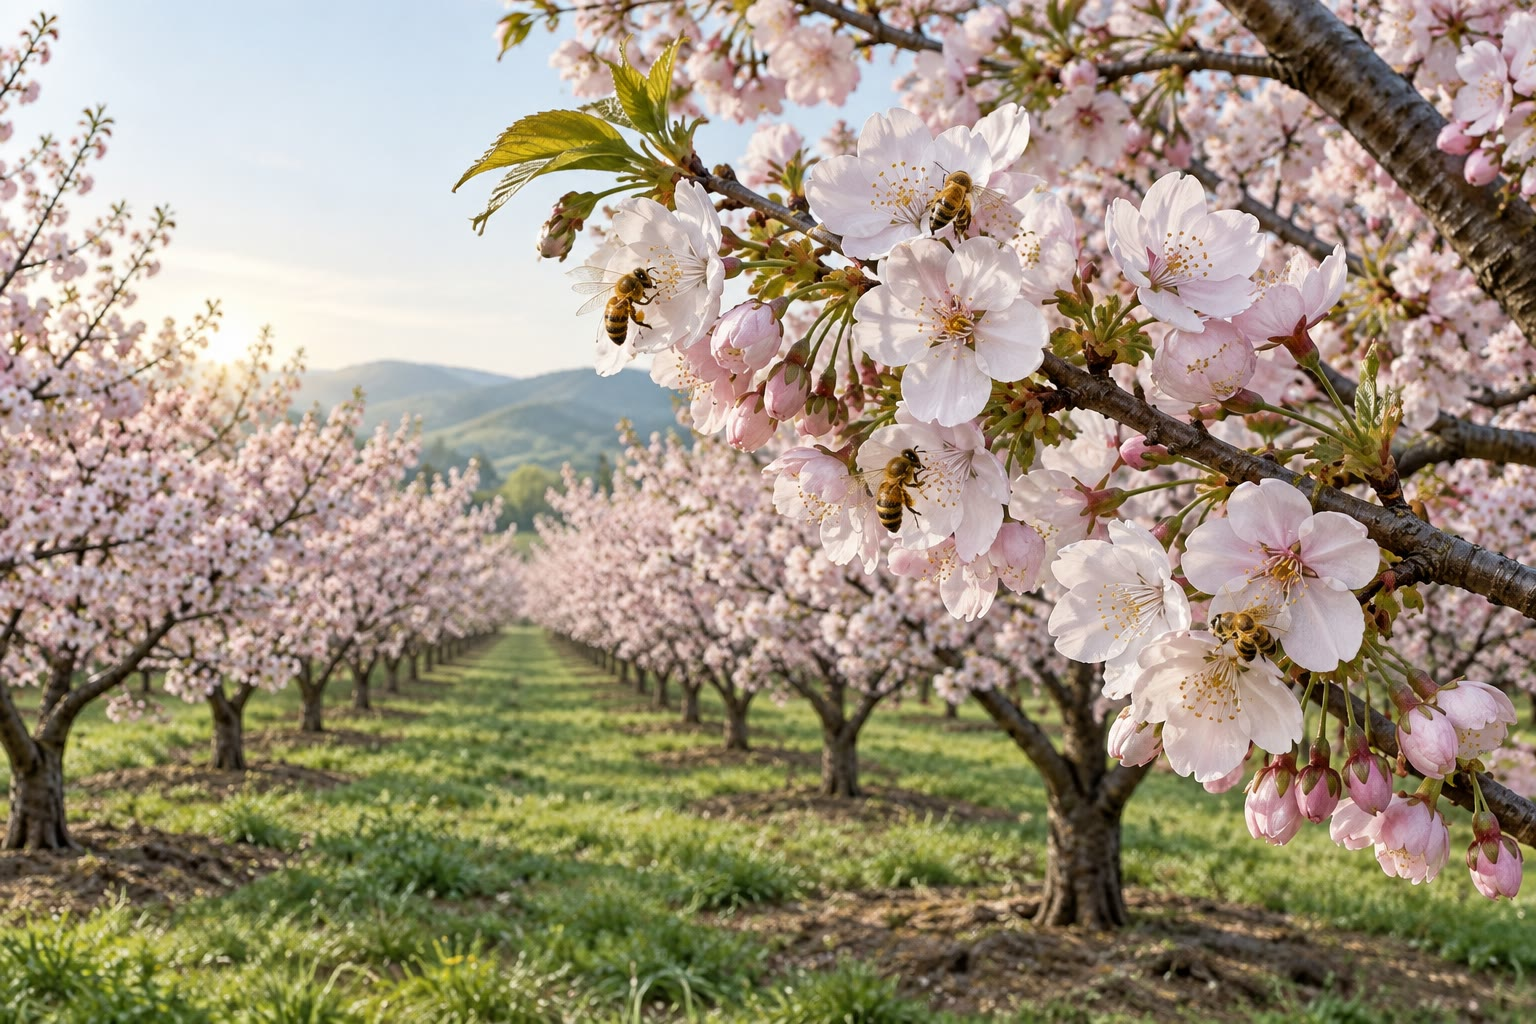
\includegraphics[width=0.62\linewidth]{images/book4/ai/b4-27-phenology-cherry.jpg}

{\small Un verger de cerisiers en \omterm{def:b2:angiosperm-reproduction:flower}{fleurs}. Les cerisiers de Kyoto, datés
dans des journaux depuis douze siècles, s'ouvrent aujourd'hui plus tôt
qu'en aucune année d'avant 1900 --- et les abeilles qui les pollinisent
doivent voler le même jour.}
\end{omfigure}

\begin{omfigure}
\begin{tikzpicture}
\begin{axis}[
  width=0.74\linewidth, height=5.4cm,
  axis x line=bottom, axis y line=left,
  xmin=0, xmax=100, ymin=0, ymax=14,
  xlabel={jours depuis le 1\textsuperscript{er} mars}, ylabel={température moyenne journalière (\unit{\celsius})},
  xlabel style={font=\small, at={(axis description cs:0.5,-0.13)}, anchor=north},
  ylabel style={font=\small},
  tick label style={font=\small}, xtick={0,20,40,60,80,100},
  legend style={font=\scriptsize, at={(0.03,0.97)}, anchor=north west, draw=none},
  clip=false,
]
\addplot[very thick, omDef, domain=0:100, samples=2] {2 + 0.1*x};
\addlegendentry{printemps avant réchauffement}
\addplot[very thick, omThm, domain=0:100, samples=2] {3 + 0.1*x};
\addlegendentry{printemps plus chaud de \qty{1}{\celsius}}
\draw[dashed, gray] (axis cs:0,5) -- (axis cs:100,5); \node[font=\scriptsize, anchor=south east] at (axis cs:100,5) {température de base $T_b = \qty{5}{\celsius}$};
\fill[omDef, opacity=0.15] (axis cs:30,5) -- (axis cs:93,5) -- (axis cs:93,11.3) -- cycle;
\fill[omThm, opacity=0.15] (axis cs:20,5) -- (axis cs:83,5) -- (axis cs:83,11.3) -- cycle;
\draw[<->, thick] (axis cs:83,1.6) -- (axis cs:93,1.6); \node[font=\scriptsize, anchor=south] at (axis cs:88,1.8) {10 jours};
\draw[dotted] (axis cs:93,0) -- (axis cs:93,5); \draw[dotted] (axis cs:83,0) -- (axis cs:83,5);
\node[font=\scriptsize, anchor=south, align=center] at (axis cs:62,11.4) {$K = 200$ degrés-jours\\ (aires grisées)};
\end{axis}
\end{tikzpicture}

{\small Les degrés-jours. L'événement se produit lorsque l'aire grisée
entre la droite de température et la base atteint $K$~; un printemps plus
chaud d'un degré franchit la base dix jours plus tôt et complète la
somme dix jours plus tôt.}
\end{omfigure}

\section{La carte~: les déplacements d'aires de répartition}

\begin{proposition}[Les isothermes se déplacent, et les espèces suivent]\label{prop:b2:global-change:range}
\index{deplacement d'aire de repartition@déplacement d'aire de répartition}\index{vitesse climatique}\index{gradient thermique vertical}
La température diminue d'environ \qty{6.5}{\celsius} par kilomètre
d'altitude et d'environ \qty{0.65}{\celsius} par centaine de kilomètres
de latitude dans la zone tempérée~; un réchauffement de \qty{1}{\celsius}
déplace donc chaque isotherme d'environ \qty{150}{m} vers le haut et de
\qty{150}{km} vers le pôle. Les espèces dont les limites sont fixées par
la température se déplacent avec leur isotherme lorsqu'elles le peuvent~:
la moyenne de centaines d'espèces étudiées s'est déplacée de \qty{11}{m}
vers le haut et de \qty{17}{km} vers le pôle par décennie depuis 1970, à
la vitesse des isothermes, et les plus rapides --- mobiles, généralistes,
à vie courte --- les devancent, tandis que les arbres, dont les \omterm{def:b2:angiosperm-reproduction:seed}{graines}
voyagent de quelques mètres par an, et les espèces déjà au sommet ou au
pôle ne peuvent pas suivre~: le sommet d'une montagne n'a nulle part où
aller, et chaque degré de réchauffement retranche les \qty{150}{m}
supérieurs de toute aire de répartition. Les espèces marines, sans
barrières et aux limites thermiques plus strictes, se déplacent le plus
vite, de plusieurs dizaines de kilomètres par décennie~; la morue, le
maquereau et les pêcheries avec eux ont remonté vers le nord à travers
des mers entières. La limite supérieure d'une aire avance, la limite
inférieure recule à mesure qu'elle se réchauffe et que de nouveaux
compétiteurs arrivent d'en dessous, et la communauté en chaque point se
recompose à partir d'espèces qui ne s'étaient jamais rencontrées.
\end{proposition}
\begin{proof}[Faits expérimentaux]
Parmesan (1996) réexamina le damier d'Édith dans son aire de l'ouest de
l'Amérique du Nord~: les populations de la limite sud et des basses
altitudes avaient disparu, celles de la limite nord et des hautes
altitudes prospéraient, et l'aire entière s'était déplacée de
\qty{92}{km} vers le nord et de \qty{124}{m} vers le haut --- la première
espèce dont on ait montré qu'elle suivait les isothermes. Lenoir et ses
collègues (2008) comparèrent des relevés de plantes forestières de
1905--1985 à ceux de 1986--2005 dans les montagnes françaises~: l'altitude
optimale de 171 espèces s'était élevée de \qty{29}{m} par décennie. Chen
et ses collègues (2011), sur deux mille espèces, trouvèrent des
déplacements deux à trois fois plus rapides que les estimations
antérieures, et proportionnels au réchauffement local.
\end{proof}

\begin{omfigure}
\begin{tikzpicture}[every node/.style={font=\scriptsize}, >=stealth]
  \fill[gray!25] (0,0) -- (3.5,4.2) -- (7,0) -- cycle;
  \draw[thick] (0,0) -- (3.5,4.2) -- (7,0);
  \foreach \y/\lab in {1.0/{\qty{12}{\celsius}}, 2.2/{\qty{8}{\celsius}}, 3.4/{\qty{4}{\celsius}}} { \draw[omDef, thick] ({\y/1.2},\y) -- ({7-\y/1.2},\y) node[right] {\lab}; }
  \foreach \y in {1.15,2.35,3.55} { \draw[omThm, thick, dashed] ({\y/1.2},\y) -- ({7-\y/1.2},\y); }
  \node[omThm, anchor=west, align=left] at (7.6,3.7) {en tirets~: les mêmes isothermes\\ après \qty{1}{\celsius} de réchauffement,\\ \qty{150}{m} plus haut};
  \fill[omProp!50] (0.83,1.0) -- (6.17,1.0) -- (5.17,2.2) -- (1.83,2.2) -- cycle;
  \node[align=center] at (3.5,1.6) {bande d'une espèce,\\ \qtyrange{1000}{1200}{m}};
  \draw[->, thick, omExo!80!black] (1.1,2.2) -- (1.1,2.9); \node[omExo!80!black, anchor=east, align=right] at (0.95,2.55) {la bande monte\\ et se rétrécit};
  \node[anchor=north] at (3.5,-0.1) {une montagne~: la surface diminue avec l'altitude, et le sommet n'a rien au-dessus de lui};
\end{tikzpicture}

{\small Un déplacement d'aire sur une montagne. Chaque degré élève les
isothermes de \qty{150}{m}~; une espèce suit sa bande vers le haut, sur
une surface plus petite, et une bande déjà au sommet disparaît.}
\end{omfigure}

\section{La mer~: acidification et chaleur}

\begin{theorem}[L'acidification]\label{thm:b2:global-change:acid}
\index{acidification des oceans@acidification des océans}\index{systeme des carbonates@système des carbonates}\index{etat de saturation@état de saturation}\index{blanchissement des coraux}
Le dioxyde de carbone qui se dissout dans l'eau de mer forme de l'acide
carbonique, qui se dissocie~: $\ensuremath{\mathrm{CO_2}} + \ensuremath{\mathrm{H_2O}} \rightleftharpoons \ensuremath{\mathrm{H^{+}}} +
\ensuremath{\mathrm{HCO_3^{-}}}$, avec $[\ensuremath{\mathrm{H^{+}}}][\ensuremath{\mathrm{HCO_3^{-}}}]/[\ensuremath{\mathrm{CO_2}}] = K_1$.
Le bicarbonate est le plus grand \omterm{def:b2:biogeochemical-cycles:reservoir}{réservoir} de carbone de l'océan et il est
maintenu presque constant par l'alcalinité, si bien que
\[
[\ensuremath{\mathrm{H^{+}}}] \propto p_{\ensuremath{\mathrm{CO_2}}}, \qquad
\Delta\mathrm{pH} \approx -\log_{10}\frac{p_{\ensuremath{\mathrm{CO_2}}}}{p_0}
\]
--- plus précisément $-0.9\log_{10}$ du rapport, car le bicarbonate
augmente un peu. De 280 à \qty{420}{ppm}, le pH de surface a baissé de
$0.15$, de $8.2$ à $8.05$~: une augmentation de \qty{40}{\%} des ions
hydrogène~; à \qty{800}{ppm}, il baisserait de $0.4$. Les ions hydrogène
supplémentaires consomment le carbonate, $\ensuremath{\mathrm{H^{+}}} + \ensuremath{\mathrm{CO_3^{2-}}} \to \ensuremath{\mathrm{HCO_3^{-}}}$, et
l'\emph{\omterm{thm:b2:global-change:acid}{état de saturation}} $\Omega$ du carbonate de calcium --- le
produit des concentrations en calcium et en carbonate divisé par le
produit de solubilité --- diminue en proportion~: les coquilles et les
squelettes d'aragonite (coraux, ptéropodes) se forment facilement pour
$\Omega > 3$, difficilement vers 1, et se dissolvent en dessous~; la
surface tropicale, à $\Omega \approx 4$ avant l'industrie et à 3
aujourd'hui, atteint 2 à
\qty{560}{ppm}, et les eaux de surface polaires, froides et riches en
\ensuremath{\mathrm{CO_2}}, atteignent 1 les premières.
\end{theorem}
\begin{proof}
D'après l'équilibre, $[\ensuremath{\mathrm{H^{+}}}] = K_1[\ensuremath{\mathrm{CO_2}}]/[\ensuremath{\mathrm{HCO_3^{-}}}]$ et
$[\ensuremath{\mathrm{CO_2}}]$ est proportionnel à $p_{\ensuremath{\mathrm{CO_2}}}$ selon la loi de Henry~;
$[\ensuremath{\mathrm{HCO_3^{-}}}]$ étant constant, $[\ensuremath{\mathrm{H^{+}}}]$ est proportionnel à
$p_{\ensuremath{\mathrm{CO_2}}}$ et $\mathrm{pH} = -\log_{10}[\ensuremath{\mathrm{H^{+}}}]$ varie de
$-\log_{10}$ du rapport. Le second équilibre, $[\ensuremath{\mathrm{H^{+}}}][\ensuremath{\mathrm{CO_3^{2-}}}]/[\ensuremath{\mathrm{HCO_3^{-}}}]
= K_2$, donne $[\ensuremath{\mathrm{CO_3^{2-}}}] \propto 1/[\ensuremath{\mathrm{H^{+}}}] \propto
1/p_{\ensuremath{\mathrm{CO_2}}}$, si bien que $\Omega$ diminue quand $p_{\ensuremath{\mathrm{CO_2}}}$ augmente, et
la hausse de \qty{40}{\%} de $[\ensuremath{\mathrm{H^{+}}}]$ correspond à une baisse de
\qty{30}{\%} du carbonate. (La chimie complète, avec la variation du
bicarbonate et les activités ioniques, donne le facteur $0.9$ et les
valeurs observées~; le volume de troisième année la traite.)
\end{proof}
\begin{proof}[Faits expérimentaux]
La station océanique située au nord d'Hawaï mesure chaque mois le pH de
surface depuis 1988~: il baisse de $0.0018$ par an, au rythme du
\ensuremath{\mathrm{CO_2}} mesuré au Mauna Loa juste au-dessus, comme l'exige la chimie.
Des ptéropodes --- les escargots de mer, nourriture des saumons et des
baleines --- récoltés au large de la côte pacifique montrent des
coquilles d'aragonite piquées et en voie de dissolution là où l'upwelling
amène en surface une eau à $\Omega <
1$. Le \omterm{thm:b2:global-change:acid}{blanchissement des coraux} est dû à la chaleur, non à l'acide~:
lorsque l'eau reste \qty{1}{\celsius} au-dessus du maximum estival
pendant quelques semaines, le corail expulse ses algues symbiotiques et
meurt de faim~; la Grande Barrière de corail a blanchi en 1998, 2002,
2016, 2017, 2020, 2022 et 2024, et la moitié de sa couverture corallienne
a disparu depuis 1995.
\end{proof}

\begin{omfigure}
\begin{tikzpicture}
\begin{axis}[
  width=0.68\linewidth, height=5.4cm,
  axis x line=bottom, axis y line=left,
  xmin=250, xmax=1000, ymin=7.6, ymax=8.3,
  xlabel={\ensuremath{\mathrm{CO_2}} atmosphérique (ppm)}, ylabel={pH de surface},
  xlabel style={font=\small, at={(axis description cs:0.5,-0.13)}, anchor=north},
  ylabel style={font=\small},
  tick label style={font=\small}, xtick={280,420,560,800,1000}, ytick={7.6,7.8,8.0,8.2},
  clip=false,
]
\addplot[very thick, omDef, domain=250:1000, samples=60] {8.2 - 0.9*log10(x/280)};
\fill[omDef] (axis cs:280,8.2) circle (2pt); \node[font=\scriptsize, anchor=south west] at (axis cs:285,8.2) {1750};
\fill[omThm] (axis cs:420,8.04) circle (2pt); \node[font=\scriptsize, anchor=south west] at (axis cs:425,8.04) {années 2020~: $-0.15$, $+\qty{40}{\%}$ \ensuremath{\mathrm{H^{+}}}};
\fill[omThm] (axis cs:800,7.79) circle (2pt); \node[font=\scriptsize, anchor=south west] at (axis cs:805,7.79) {2100 avec des émissions élevées};
\node[font=\scriptsize, anchor=north east, align=right] at (axis cs:1000,8.28) {$\Omega_{\text{aragonite}}$, tropiques~:\\ 4 en 1750, 3 aujourd'hui, 2 à \qty{560}{ppm}};
\end{axis}
\end{tikzpicture}

{\small pH de l'océan de surface en fonction du dioxyde de carbone
atmosphérique,
$\mathrm{pH} = 8.2 - 0.9\log_{10}(p/280)$. L'échelle est
logarithmique~: chaque dixième d'unité correspond à un quart d'ions
hydrogène en plus.}
\end{omfigure}

\begin{omfigure}
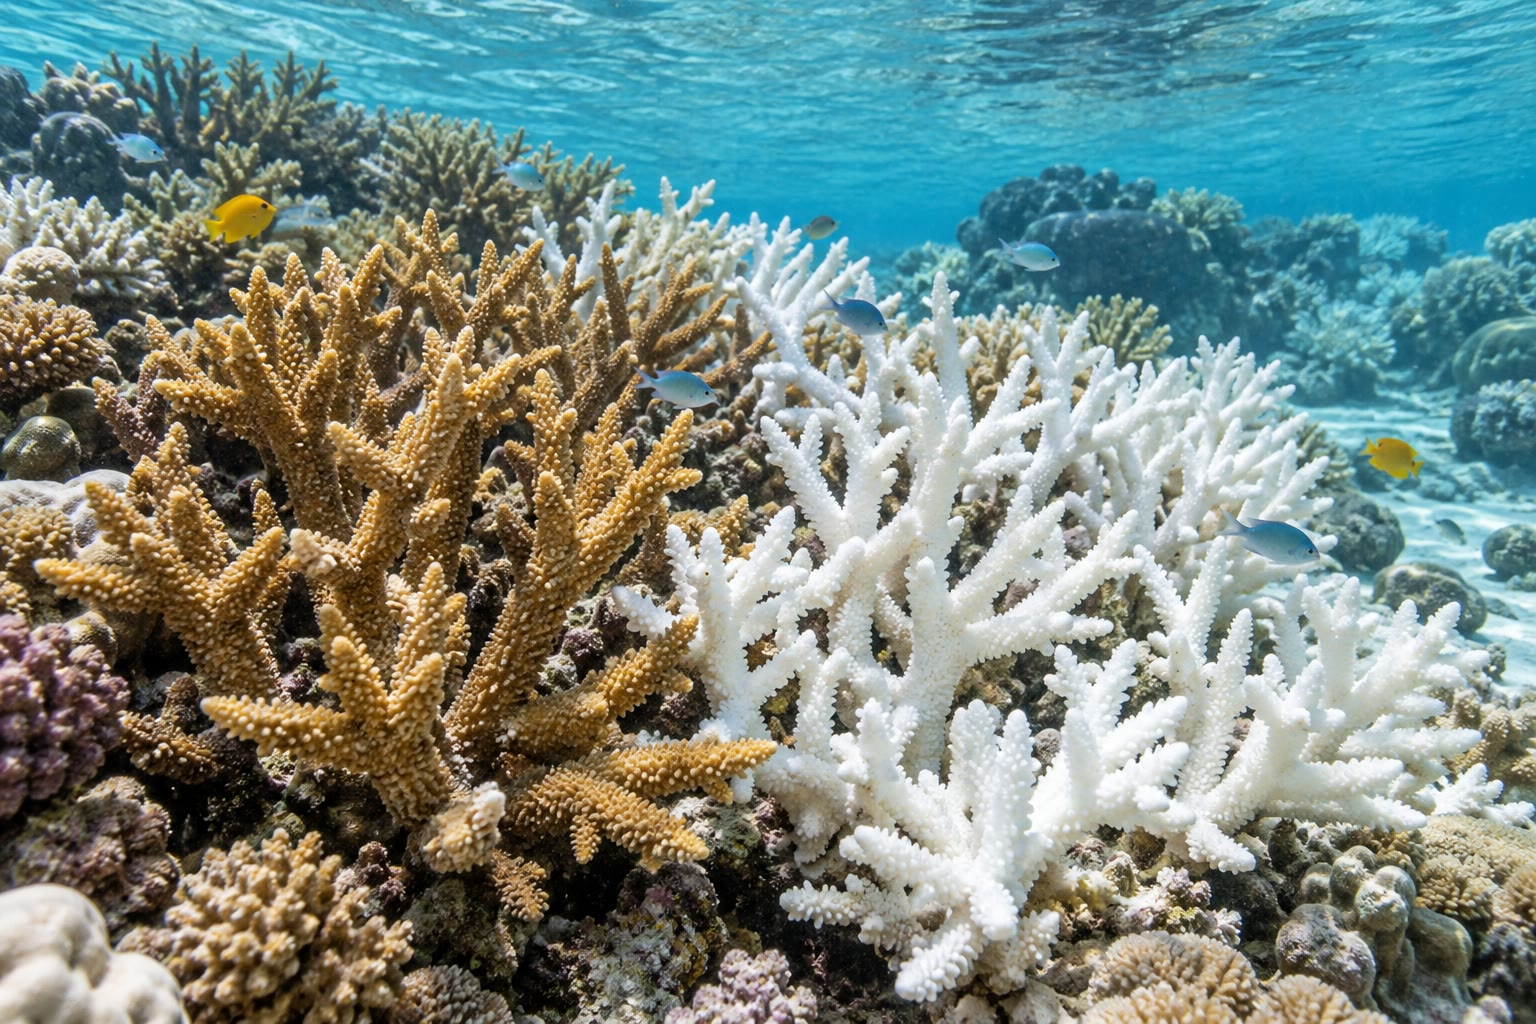
\includegraphics[width=0.44\linewidth]{images/book4/ai/b4-27-coral-bleaching.jpg}\hspace{0.04\linewidth}
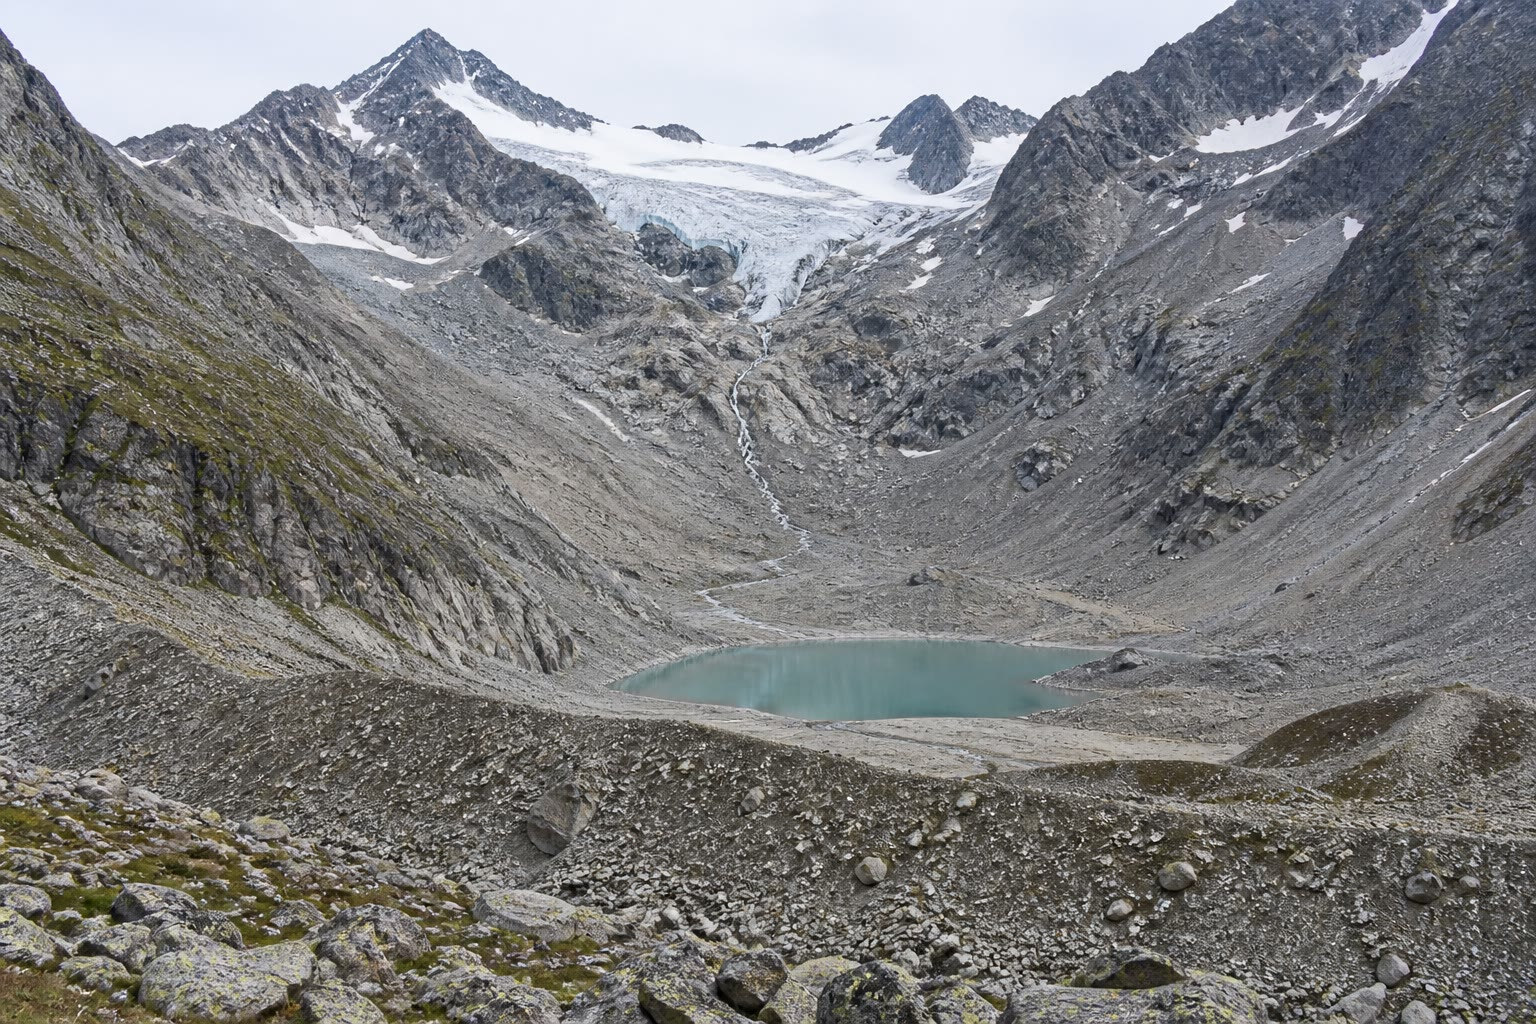
\includegraphics[width=0.44\linewidth]{images/book4/ai/b4-27-glacier-retreat.jpg}

{\small Deux thermomètres. À gauche~: un récif blanchi, le squelette
blanc du corail apparaissant à travers des tissus qui ont perdu leurs
algues. À droite~: un glacier de vallée qui a reculé vers l'amont,
laissant la roche nue là où se trouvait la glace il y a un siècle.}
\end{omfigure}

\section{Le bilan~: l'extinction et son estimation}

\begin{theorem}[La relation aire--espèces et le coût de la perte d'habitat]\label{thm:b2:global-change:sar}
\index{relation aire--especes@relation aire--espèces}\index{taux d'extinction}\index{perte d'habitat}\index{dette d'extinction}
Le nombre d'espèces trouvées sur une aire $A$ croît comme une puissance de
l'aire, $S = cA^{z}$, avec $z \approx 0.25$ pour les îles et les
fragments d'habitat (doubler l'aire ajoute un cinquième d'espèces~; une
aire cent fois plus grande, trois fois plus d'espèces). Si un habitat est
réduit à une fraction $1 - h$ de son étendue, le nombre d'espèces qu'il
peut finalement accueillir tombe à $(1 - h)^{z}$ du nombre initial~: la
perte de la moitié de l'habitat coûte \qty{16}{\%} de ses espèces,
celle de \qty{90}{\%} en coûte \qty{44}{\%}, et celle de \qty{99}{\%}
\qty{68}{\%}. La perte n'est pas immédiate --- les survivants du
fragment persistent un temps, une \emph{\omterm{thm:b2:global-change:sar}{dette d'extinction}} payée au fil
des décennies à mesure que de petites populations succombent à la dérive
et à la consanguinité du
\cref{ch:b2:population-genetics} --- et elle fonde l'estimation selon
laquelle le \omterm{thm:b2:global-change:sar}{taux d'extinction} actuel vaut cent à mille fois le taux de
fond des archives fossiles~: environ une espèce sur un million par an,
contre plusieurs milliers par an, sur quelque dix millions, qui
disparaissent aujourd'hui.
\end{theorem}
\begin{proof}
$S'/S = (A'/A)^{z} = (1 - h)^{z}$~; avec $z = 0.25$, $0.5^{0.25} =
0.84$, $0.1^{0.25} = 0.56$, $0.01^{0.25} = 0.32$. La relation
elle-même est empirique~; son exposant traduit l'équilibre, sur les îles,
entre l'immigration de nouvelles espèces (qui diminue à mesure que l'île
se remplit) et l'extinction des espèces résidentes (qui augmente à mesure
que leurs populations diminuent avec l'aire), l'équilibre de la théorie
de MacArthur et Wilson.
\end{proof}
\begin{proof}[Faits expérimentaux]
Les îles de l'archipel du Krakatoa, stérilisées par l'éruption de
1883, furent recolonisées par des plantes, des oiseaux et des insectes
selon une succession qui atteignit, en cinquante ans, les nombres
d'espèces prédits d'après leurs aires~; les îlots de mangrove que
Simberloff et Wilson fumigèrent en Floride en 1966 retrouvèrent leur
nombre d'espèces initial, avec des espèces différentes, en un an. La
forêt atlantique du Brésil, réduite à \qty{10}{\%} de son étendue, a
perdu ou presque perdu la fraction de ses espèces d'oiseaux que prédit la
relation~; et dans tous les groupes évalués par l'Union internationale
pour la conservation de la nature, d'un quart à un tiers des espèces sont
menacées --- oiseaux \qty{13}{\%}, mammifères \qty{27}{\%}, amphibiens
\qty{41}{\%}, coraux
\qty{44}{\%} --- la \omterm{thm:b2:global-change:sar}{perte d'habitat} étant la première cause, et la chasse,
les \omterm{prop:b2:global-change:invasion}{espèces invasives}, la pollution et, de plus en plus, le climat les
autres.
\end{proof}

\begin{omfigure}
\begin{tikzpicture}
\begin{loglogaxis}[
  width=0.68\linewidth, height=5.4cm,
  axis x line=bottom, axis y line=left,
  xmin=1, xmax=100000, ymin=5, ymax=200,
  xlabel={aire de l'île (\unit{km^2})}, ylabel={espèces d'oiseaux terrestres},
  xlabel style={font=\small, at={(axis description cs:0.5,-0.13)}, anchor=north},
  ylabel style={font=\small},
  tick label style={font=\small},
  clip=false,
]
\addplot[only marks, mark=*, mark size=2pt, omDef] coordinates {(1.5,9) (8,14) (35,22) (150,32) (400,37) (1200,52) (4000,70) (13000,92) (35000,125) (85000,160)};
\addplot[very thick, omThm, domain=1:100000, samples=2] {9*x^0.25};
\node[font=\scriptsize, omThm, anchor=north west, align=left] at (axis cs:2,120) {$S = 9A^{0.25}$~: une aire cent\\ fois plus grande, trois fois\\ plus d'espèces};
\end{loglogaxis}
\end{tikzpicture}

{\small La \omterm{thm:b2:global-change:sar}{relation aire--espèces}, ici pour les oiseaux terrestres des
îles d'un archipel~: une droite de pente $z = 0.25$ en coordonnées
logarithmiques. Réduisez un habitat au dixième et il ne conservera, à
terme, guère plus de la moitié de ses espèces.}
\end{omfigure}

\begin{proposition}[Invasions, services, et ce qui peut être fait]\label{prop:b2:global-change:invasion}
\index{espece invasive@espèce invasive}\index{services ecosystemiques@services écosystémiques}\index{attenuation@atténuation}\index{neutralite carbone@neutralité carbone}
Les navires, les avions et le commerce ont fait franchir à des milliers
d'espèces les barrières qui les tenaient séparées~; la plupart ne
parviennent pas à s'établir, mais les quelques-unes qui y parviennent ---
le lapin en Australie, la moule zébrée dans les Grands Lacs, le serpent
brun arboricole qui a vidé Guam de ses oiseaux, le champignon chytride
qui a conduit quatre-vingt-dix espèces d'amphibiens à l'extinction ---
s'étendent en un front qui avance à vitesse constante, $c =
2\sqrt{rD}$ pour une population qui croît au taux $r$ et se disperse
avec un coefficient de diffusion $D$ (le rat musqué de Skellam, lâché
près de Prague en 1905, s'est répandu à travers l'Europe à raison de
\qty{11}{km} par an, le rayon de son aire croissant linéairement avec le
temps). Face à tout cela se tient ce que la biosphère fait pour sa seule
espèce encombrante~: la \omterm{def:b2:angiosperm-reproduction:pollination}{pollinisation} des trois quarts des cultures,
l'épuration de l'eau, la régulation des crues, la \omterm{prop:b2:biogeochemical-cycles:nitrogen}{fixation de l'azote} et
la fabrication du \omterm{def:b2:living-soil:soil}{sol}, les pêcheries, le carbone stocké dans les forêts
et les \omterm{def:b2:living-soil:soil}{sols} --- des \emph{\omterm{prop:b2:global-change:invasion}{services écosystémiques}} évalués, là où l'on
peut leur fixer un prix, à plus que le produit économique mondial. Ce qui
peut être fait découle des chiffres.
Le réchauffement s'arrête quand les émissions nettes s'arrêtent, et pas
avant~: les modèles à compartiments du
\cref{ch:b2:biogeochemical-cycles} ne permettent aucune autre lecture de
la \emph{\omterm{prop:b2:global-change:invasion}{neutralité carbone}}. Les terres peuvent aider, dans certaines
limites --- une gigatonne de carbone par an grâce au reboisement et aux
\omterm{def:b2:living-soil:soil}{sols} pendant quelques décennies, contre dix issues des combustibles
fossiles --- et l'on peut aider les espèces à se déplacer, ou les
conserver dans des réserves assez grandes et assez connectées pour que
la \omterm{thm:b2:global-change:sar}{relation aire--espèces} et la dérive des petites populations ne les
achèvent pas. Les outils sont ceux de ce livre~: la \omterm{def:b2:population-genetics:frequencies}{génétique des
populations} de la réserve, la compétition de l'envahisseur, la
phénologie de la culture, le bilan du \omterm{def:b2:living-soil:soil}{sol}.
\end{proposition}

\begin{example}[Trois avenirs]\label{ex:b2:global-change:scenarios}
Des émissions maintenues à \qty{10}{GtC} par an jusqu'en 2100 ajoutent
\qty{800}{GtC} aux \qty{700}{} déjà émises~: $1.65\times 1.5 =
\qty{2.5}{\celsius}$ à la fin du siècle, et la hausse continue. Des
émissions ramenées à zéro en 2070 ajoutent environ \qty{250}{GtC}~:
\qty{1.6}{\celsius}, puis un plateau. Doubler d'abord les émissions, comme
l'ont fait les premières décennies du siècle, donne \qty{4}{\celsius} ou
plus. Les aires de répartition de la zone tempérée se déplacent de
\qty{200}{km} au-delà de leur position actuelle dans le premier cas et
de \qty{60}{km} dans le second~; le printemps arrive vingt-cinq jours
plus tôt, ou six~; le pH de surface atteint $7.8$, ou reste voisin de
$8.0$~; et les estimations d'extinction, qui dépendent à la fois de
l'habitat et du réchauffement, vont d'un dixième à un tiers des espèces.
La différence entre ces avenirs est l'aire cumulée sous une courbe,
c'est-à-dire la somme de décisions qui n'ont pas encore été prises.
\end{example}

\section{Exercices}

\begin{exercise}[$\star$]\label{exo:b2:global-change:1}
Énoncer la relation entre réchauffement et \omterm{prop:b2:global-change:tcre}{émissions cumulées}, et
calculer le réchauffement pour des \omterm{prop:b2:global-change:tcre}{émissions cumulées} de 700, 1000 et
\qty{2000}{GtC}.
\end{exercise}

\begin{exercise}[$\star$]\label{exo:b2:global-change:2}
Définir degrés-jours et \omterm{thm:b2:global-change:phenology}{décalage phénologique}, en prenant le gobemouche
comme exemple.
\end{exercise}

\begin{exercise}[$\star$]\label{exo:b2:global-change:3}
De combien les isothermes se déplacent-ils vers le haut et vers le pôle
par degré de réchauffement, et pourquoi une espèce de sommet ne peut-elle
pas suivre~?
\end{exercise}

\begin{exercise}[$\star$]\label{exo:b2:global-change:4}
Expliquer en trois phrases pourquoi l'ajout de \ensuremath{\mathrm{CO_2}} à la mer abaisse
son pH et sa teneur en carbonate, et quels organismes en souffrent.
\end{exercise}

\begin{exercise}[$\star\star$]\label{exo:b2:global-change:5}
Calculer le \omterm{prop:b2:global-change:tcre}{budget carbone} restant pour \qty{1.5}{\celsius} et pour
\qty{2}{\celsius} avec $\lambda = \qty{1.65}{\celsius}$ par
\qty{1000}{GtC} et \qty{700}{GtC} déjà émises~; convertir les deux en
années à \qty{10}{GtC/yr}.
\end{exercise}

\begin{exercise}[$\star\star$]\label{exo:b2:global-change:6}
Le printemps se réchauffe de $b = \qty{0.12}{\celsius}$ par jour à partir
d'une base de
\qty{5}{\celsius}~; un papillon de nuit a besoin de $K = 150$ degrés-jours.
Calculer le nombre de jours entre le franchissement de la base et
l'émergence, et l'avancée pour un réchauffement de \qty{1.5}{\celsius}.
\end{exercise}

\begin{exercise}[$\star\star$]\label{exo:b2:global-change:7}
L'aire d'une plante s'étend de \qtyrange{800}{1400}{m} sur une montagne
de \qty{1800}{m} dont la surface diminue de moitié tous les \qty{300}{m}
d'altitude. Après \qty{3}{\celsius} de réchauffement, où se trouve la
bande et quelle surface a-t-elle perdue~? Après \qty{5}{\celsius}~?
\end{exercise}

\begin{exercise}[$\star\star$]\label{exo:b2:global-change:8}
Calculer le pH de surface et la hausse de la concentration en ions
hydrogène à 560, 800 et \qty{1000}{ppm}, à partir de $\mathrm{pH} = 8.2 -
0.9\log_{10}(p/280)$.
\end{exercise}

\begin{exercise}[$\star\star$]\label{exo:b2:global-change:9}
Avec $z = 0.25$, quelle fraction des espèces finit par être perdue
lorsque \qty{70}{\%}, \qty{95}{\%} et \qty{99.9}{\%} d'un habitat sont
détruits~? Pourquoi la perte immédiate est-elle plus faible~?
\end{exercise}

\begin{exercise}[$\star\star\star$]\label{exo:b2:global-change:10}
Une espèce envahissante croît au taux $r = 0.7$ par an et se disperse
avec $D =
\qty{20}{km^2/yr}$. Calculer la vitesse de son front et le temps
nécessaire pour traverser un pays de \qty{1000}{km} de large. Qu'est-ce
qui divise la vitesse par deux~: diviser $r$ par deux ou diviser $D$ par
deux~?
\end{exercise}

\begin{exercise}[$\star\star\star$]\label{exo:b2:global-change:11}
Le \omterm{thm:b2:global-change:sar}{taux d'extinction} de fond est d'une extinction par million
d'espèces-années et il existe 8 millions d'espèces. Calculer le nombre
attendu d'extinctions par an et par siècle au taux de fond, et à mille
fois ce taux. Comparer aux dix mille extinctions documentées au cours du
dernier siècle et commenter l'écart.
\end{exercise}

\begin{exercise}[$\star\star\star$]\label{exo:b2:global-change:12}
«~Le réchauffement s'arrête quand les émissions nettes s'arrêtent.~»
Justifier à partir du \omterm{thm:b2:biogeochemical-cycles:box}{modèle à un compartiment} de l'atmosphère et de la
proportionnalité du réchauffement aux \omterm{prop:b2:global-change:tcre}{émissions cumulées}, et dire ce qui
manque à l'argument.
\end{exercise}

\section{Problème~: la biosphère en 2100}

\begin{problem}[{Problème du week-end --- deux trajectoires d'émissions
menées jusqu'en 2100~: le réchauffement de chacune, le printemps qu'elle
produit, la distance que parcourent ses isothermes, l'acide qu'elle met
dans la mer et les espèces qu'elle coûte à une forêt, jusqu'aux deux
réchauffements, aux deux valeurs de pH et à la fraction d'espèces
perdues}]
\label{pb:b2:global-change:1}
Données. $\lambda = \qty{1.65}{\celsius}$ par \qty{1000}{GtC}~;
\qty{700}{GtC} émises en 2020 (réchauffement \qty{1.2}{\celsius}).
Trajectoire A~: \qty{10}{GtC/yr} constants jusqu'en 2100. Trajectoire B~:
décroissance linéaire jusqu'à zéro en 2070. Le printemps se réchauffe de
$b = \qty{0.1}{\celsius}$ par jour au-dessus d'une base de
\qty{5}{\celsius}~; un arbre a besoin de $K = 200$ degrés-jours pour
débourrer, et un oiseau migrateur arrive à date fixe, 20 jours après la
feuillaison de l'arbre en 2020. \omterm{prop:b2:global-change:range}{Gradient thermique vertical}
\qty{6.5}{\celsius/km}~; gradient latitudinal \qty{0.65}{\celsius} par
\qty{100}{km}. Océan~: $\mathrm{pH} = 8.2 - 0.9\log_{10}(p/280)$~;
\ensuremath{\mathrm{CO_2}} en 2100~: \qty{600}{ppm} sur la trajectoire A,
\qty{420}{ppm} sur la trajectoire B.
Une région forestière de \qty{e5}{km^2} comptant 400 espèces d'arbres,
avec $z = 0.25$, perd \qty{60}{\%} de sa surface par défrichement d'ici
2100 sur la trajectoire A et
\qty{20}{\%} sur la trajectoire B.

\medskip
\noindent\textbf{Partie I --- Le réchauffement.}
\begin{enumerate}
  \item Calculer les \omterm{prop:b2:global-change:tcre}{émissions cumulées} en 2100 sur chaque trajectoire.
  \item Calculer le réchauffement en 2100 sur chaque trajectoire.
  \item Calculer le réchauffement en 2050 sur chacune.
  \item Quelle est la vitesse de réchauffement par décennie sur la
        trajectoire A~? Comparer aux \qty{0.2}{\celsius} par décennie
        observés.
  \item Sur la trajectoire B, le réchauffement s'arrête-t-il en 2070~?
        Pourquoi, d'après la proportionnalité~?
  \item Quelles \omterm{prop:b2:global-change:tcre}{émissions cumulées} correspondent à \qty{2}{\celsius}, et
        en quelle année la trajectoire A les atteint-elle~?
\end{enumerate}

\medskip
\noindent\textbf{Partie II --- Le printemps.}
\begin{enumerate}[resume]
  \item Calculer le nombre de jours entre le franchissement de la base et
        la feuillaison en 2020.
  \item Calculer l'avancée de la feuillaison par rapport à 2020, en 2100,
        sur chaque trajectoire (réchauffement compté à partir de 2020).
  \item La date d'arrivée de l'oiseau ne change pas. Calculer l'écart
        entre feuillaison et arrivée sur chaque trajectoire en 2100.
  \item Les chenilles dont l'oiseau a besoin culminent 15 jours après la
        feuillaison et durent 10 jours. Sur quelle trajectoire l'oiseau
        les trouve-t-il encore~?
  \item Supposons au contraire que l'oiseau avance de \qty{3}{d} par
        degré. Recalculer l'écart sur la trajectoire A.
  \item Expliquer en une phrase pourquoi c'est le décalage, et non le
        réchauffement lui-même, qui menace l'oiseau.
\end{enumerate}

\medskip
\noindent\textbf{Partie III --- Les aires de répartition.}
\begin{enumerate}[resume]
  \item Calculer le déplacement en altitude et en latitude des isothermes
        sur chaque trajectoire, par rapport à 2020.
  \item Une espèce d'arbre se disperse de \qty{100}{m} par an. Peut-elle
        suivre les isothermes vers le pôle sur la trajectoire A~? Sur la
        trajectoire B~?
  \item Une espèce occupe \qtyrange{1500}{1800}{m} sur une montagne de
        \qty{2000}{m}. Sur la trajectoire A, où se situe sa bande en 2100,
        et que se passe-t-il~?
  \item La surface de la montagne diminue de moitié tous les \qty{300}{m}.
        Calculer le facteur de surface perdu par cette espèce sur la
        trajectoire B.
  \item Un poisson marin suit les isothermes à \qty{30}{km} par décennie.
        Est-ce suffisant sur la trajectoire A~?
  \item Expliquer pourquoi la limite inférieure d'une aire recule même là
        où l'espèce pourrait tolérer la chaleur.
\end{enumerate}

\medskip
\noindent\textbf{Partie IV --- La mer et la forêt.}
\begin{enumerate}[resume]
  \item Calculer le pH de surface en 2100 sur chaque trajectoire, et la
        hausse de la concentration en ions hydrogène depuis 1750.
  \item L'\omterm{thm:b2:global-change:acid}{état de saturation} $\Omega$ de la surface tropicale valait
        4 en 1750 et varie comme $[\ensuremath{\mathrm{H^{+}}}]^{-1}$. Le calculer en 2100
        sur chaque trajectoire et dire ce que cela signifie pour les coraux.
  \item Calculer le nombre d'espèces d'arbres que la région forestière
        peut finalement accueillir sur chaque trajectoire, et le nombre
        perdu.
  \item Le réchauffement ajoute des pertes~: supposons que chaque degré
        au-dessus de 2020 retire encore \qty{5}{\%} des espèces
        survivantes. Recalculer les espèces restantes sur chaque
        trajectoire.
  \item Donner la fraction des 400 espèces perdues sur chaque trajectoire.
  \item Laquelle des deux causes, le défrichement ou le réchauffement,
        domine sur chaque trajectoire~?
  \item Énoncer le résultat~: le réchauffement, le pH et la fraction
        d'espèces d'arbres perdues en 2100 sur chaque trajectoire.
\end{enumerate}
\end{problem}
